\documentclass{standalone}
\usepackage{tikz}
\usepackage{ctex,siunitx}
\setCJKmainfont{Noto Serif CJK SC}
\usepackage{tkz-euclide}
\usepackage{amsmath}
\usetikzlibrary{patterns, calc}
\usetikzlibrary {decorations.pathmorphing, decorations.pathreplacing, decorations.shapes,}

\begin{document}
\small
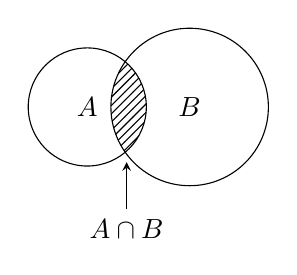
\begin{tikzpicture}[>=stealth,scale=1.0]
  \tkzSetUpPoint[fill=black]
  % \useasboundingbox(-1,-0.75)rectangle(3.7,1.4);
  \draw (0,0)node{$A$} circle(.75);
  \draw (1.3,0)node{$B$} circle (1);
  \draw[->](.5,-1.3)node[below]{$A\cap B$}--(.5,-.7);
  \clip {(0,0) circle (.75)};
  \fill[pattern=north east lines] {(1.3,0) circle (1)};
\end{tikzpicture}
\end{document}